%!TEX root = ../var.tex
\textbf{Теорема Пуассона}

\begin{zam}
По теор. 9.2 вероятность появления $k$ успехов при $n$
испытаниях схемы Бернулли с вероятностью успеха равной p вычисляется по формуле

$$\P(\xi_n = k) = C_n^k p^k (1 − p)^{n−k} = C_n^k p^k q^{n−k}.$$

Если числа $k$ и $n$ большие и при этом одна из вероятностей $p$ или $q$ мала, то подсчёт по этой формуле становится очень трудным. Мы рассмотрим три случая, когда для упрощения вычислений применимы приближённые формулы.
\end{zam}

\begin{definition}
Дискретная случайная величина $\xi$ со счётным пространством $\Omega = \{ 0, 1, 2, \ldots , k, \ldots , \}$, подчиняется распределению Пуассона с параметром $\lambda > 0$, если её ряд распределения определена соответствием $k \to \P_{\lambda} (k) = \frac{\lambda^k}{k!}e^{−\lambda}$. (Ср. с опред 4.11.)
\end{definition}

Нетрудно подсчитать, что для распределения Пуассона $\M \xi = \lambda$ и $\D \xi = \lambda$. На рис. 25 показаны функции $\P_{\lambda} (k)$ для $\lambda = 0, 1; 1; 10$, где пунктиром показаны огибающие. В каждом случае сумма длин вертикальных отрезков равна 1. Сравните график на рис. 25.3 с графиком биномиального распределения, показанным на рис. 8: обе случайные величины имеют близкие математические ожидания и похожие графики, только биномиальный график -- без <<хвоста>>. Эта внешняя схожесть наводит на мысль, что биномиальное распределение может быть аппроксимировано распределением
Пуассона.

\begin{figure}[H]
	\centering
	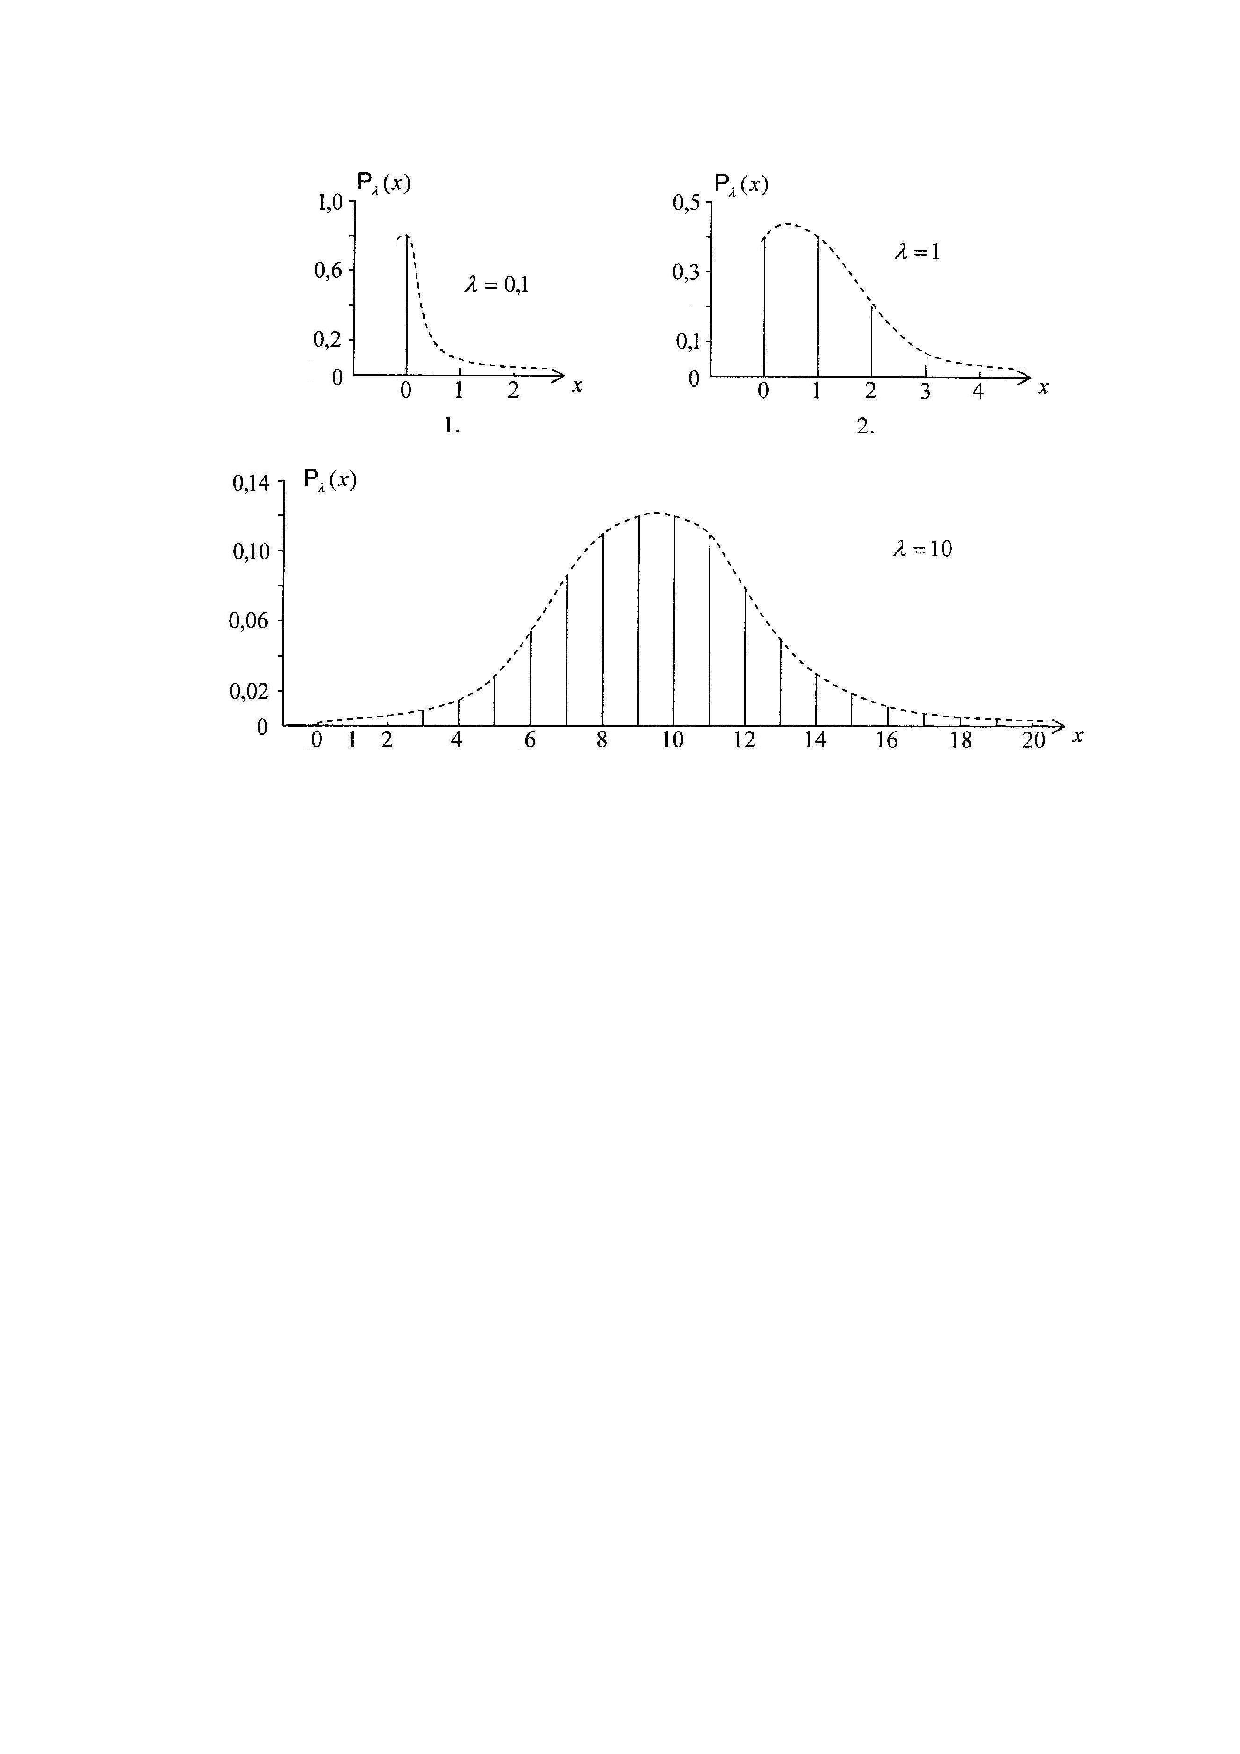
\includegraphics[]{pic/pic25}
	\caption{Распределение Пуассона}
	\label{fig25}
\end{figure} 
Рассмотрим бесконечную таблицу событий:
$$\begin{matrix} 
A_{11} &  &  &  &  \\
A_{21} & A_{22} &  &  &  \\
A_{31} & A_{32} & A_{33} &  &  \\
\ldots & \ldots & \ldots & \ldots &  \\
A_{n1} & A_{n2} & A_{n3} & \ldots & A_{nn}\\
\ldots & \ldots & \ldots & \ldots & \ldots\\   
\end{matrix}$$

где 1) в $n$-ой строке, $n = 1, 2, \ldots$ , стоят $n$ событий $A_{n1} , A_{n2} , A_{n3} , \ldots , A_{nn}$ ;
2) в каждой строке события попарно независимы;
3) каждое событие в $n$-ой строке происходит с одной и той же вероятностью $p_n$ , зависящей только от номера строки.
Обозначим через $\xi_n$ случайную величину, равную числу событий $A_{ni}$ , произошедших в $n$-ой строке. Ясно, что случайная величина $\xi_n$ принимает значения $k = 0, 1, 2, \ldots , n$ и имеет биномиальное распределение $k \to C_n^k p^k_n (1 − pn )^{n−k}.$

\begin{definition}
Говорят, что последовательность $p1 , p2 , \ldots ,
pn , \ldots$ удовлетворяет закону малых чисел, если $\lim\limits_{n \to \infty} p_n = 0$ и существуnет предел
$$\lim\limits_{n \to \infty} np_n = \lambda, \quad \text{где} \quad  0 < \lambda < \infty.$$
\end{definition}

\begin{theorem}[Пуассона]
Если последовательность $\{ p_n\}_{n=1}^{\infty}$удовлетворяет закону малых чисел, то для любого $k \geq 0$ имеет место равенство
$$\lim\limits_{n \to \infty} C_n^k p_n^k (1-p_n)^{n-k} = \frac{\lambda^k}{k!}e^{-\lambda}$$
\end{theorem}

\begin{proof}
Обозначим $\lambda_n = n \cdot p_n$ . Тогда

\begin{gather*}
	\P = (\xi_n = k) = C_n^k p_n^k (1 - p_n)^{n-k} =\\= 
	\frac{n(n-1) \ldots (n-k+1)}{k!}
	\left( \frac{\lambda_n}{n} \right)^k
	\left( 1 - \frac{\lambda_n}{n} \right)^{n-k} =\\=
	\frac{\lambda_n^k}{k!}\cdot
	\frac{n(n-1) \ldots (n-k+1)}{n^k}
	\left( 1 - \frac{\lambda_n}{n} \right)^{n}
	\left( 1 - \frac{\lambda_n}{n} \right)^{-k} =\\=
    \frac{\lambda^k_n}{k!} \left( 1 - \frac{1}{n} \right) \left( 1 - \frac{2}{n} \right) \ldots \left( 1 - \frac{k-1}{n} \right) \left( 1 - \frac{\lambda_n}{n} \right)^n \left( 1 - \frac{\lambda_n}{n} \right)^{-k}.
\end{gather*}

Отсюда переходя к пределу при $n \to \infty$ получим требуемый результат.
 \end{proof}

 \begin{zam}
Теорема Пуассона доставляет приближённую формулу

$$\P(\xi_n = k) = C^k_n p^k (1 − p_n )^{n−k} \approx \frac{(np)^k}{k!}e^{-np}$$

Заметим, что в примере 23.9.2) мы вычислили математическое ожидание и дисперсию для биномиального распределения $\M \xi = np$ и $\D \xi = npq$.
Поэтому имеем

$$\P(\xi_n = k) \approx \frac{(\M \xi)^k}{k!}e^{-\M \xi}.$$

Параметр $\lambda = np$ является математическим ожиданием для распределения Пуассона. Таким образом, биномиальное распределение аппроксимируется распределением Пуассона так, что оба распределения имеют одно и то же математическое ожидание. На самом деле оба распределения имеют и достаточно близкие дисперсии. В области применения приближённой формулы вероятность $p$ должна быть мала, а значит $q = 1 − p \approx 1$, поэтому
$\D \xi = npq \approx np = \lambda$. 	
 \end{zam}

\textbf{Пример.} Вероятность попадания в цель при каждом выстреле равна 0,001. Найти вероятность попадания в цель двумя и более пулями, если число выстрелов равно 5 000.
Решение. Этот эксперимент реализует схему Бернулли, и использование точной формулы даёт значение искомой вероятности равное
\begin{gather}
	\label{pisk}
	\P(\xi_n \geq 2) = \sum\limits_{k=2}^{5000} \P(\xi_{5000} = k) =\\=
	1 - \P(\xi_{5000} = 0) - \P(\xi_{5000} = 1) =\\=
	1 − 0, 999^{5000} − 5000 \cdot 0, 001 \cdot 0, 999^{4999} .
\end{gather}
Воспользуемся теоремой Пуассона $\P(\xi_n = k) \approx \frac{(np)^k}{k!}e^{-np}$. 
Вычислим: $\lambda = np = 5000 \cdot 0, 001 = 5, \P(\xi_{5000} = 0) \approx e^{-5} , \P(\xi_{5000} = 1) \approx 5e^{−5}.$ 
Поэтому
$$\P_n (\xi \geq 2) = 1 − \P(\xi_{5000} = 0) − \P(\xi_{5000} = 1) \approx 1 − 6e^{−5} \approx 0, 9596.$$
Вычисление по точной формуле (\ref{pisk}) с точностью до четвёртого знака даёт ответ $P_n (\xi \geq 2) = 0, 9575$. Нетрудно подсчитать, что ошибка от применения приближённой формулы составляет меньше 0,25\%.

\textbf{Теорема Муавра}. Эта предельная теорема обеспечивает приближённое вычисление вероятностей биномиального распределения,

$$\P(\xi_n = k) = C^k_n \cdot pk \cdot q^{n−k},$$

в случае, когда при $n \to \infty$ обе величины $k \to \infty$ и $n − k \to \infty$ так, что величина $x_k = \frac{k - np}{\sqrt{npq}}$ ограничена, т.е. существует $N > 0$, такое что $|x_k| < N$ для $k = 0, 1, 2, \ldots .$

\begin{theorem}[Локальная теорема Муавра\footnote{
Абрахам де Муавр (Abraham de Moivre, 1667 — 1754), английский математик французского происхождения. Основные труды по теории рядов, теории вероятностей, теории комплексных чисел.	
}]
Если вероятность $0 < p < 1$ постоянна, и величина $x_k = \frac{k - np}{\sqrt{npq}}$ ограничена, то справедлива формула
$$\lim\limits_{n \to \infty} 
\left[ C_n^k p^k q^{n-k} - \frac{1}{\sqrt{2\pi npq}} 
exp \left(-\frac{x_k^2}{2} \right) \right] = 0$$
(Без доказательства.)
\end{theorem}

\begin{zam}
Локальная теорема Муавра доставляет приближённую формулу
$$\P(\xi_n = k) = C_n^k p^k q^{n-k} \approx \frac{1}{\sqrt{2\pi npq}} exp \left(-\frac{x_k^2}{2} \right)$$

Напомним, что в примере 18.9.2) мы вычислили математическое ожидание и дисперсию для биномиального распределения $\M \xi = np$ и $\D \xi = npq$.
Поэтому имеем

\begin{gather*}
	x_k = \frac{k - np}{\sqrt{npq}}  = \frac{k - \M \xi}{\sqrt{\D \xi}} = \frac{K - \M \xi}{\sigma} \text{и}\\
	\P(\xi_n = k) \approx \frac{1}{\sigma \sqrt{2\pi}} exp \left(-\frac{(k - \M \xi)^2}{2 \sigma^2} \right) 
\end{gather*}

Последняя формула означает, что биномиальное распределение аппроксимировано нормальным, причём оба распределения имеют одинаковые математические ожидания и дисперсии.
\end{zam}

\textbf{Пример.}
Пусть надо вычислить $\P(\xi_n = k)$ при $n = 10 000, k = 40, p = 0, 005$. Сделаем подготовительные вычисления:

$$\sqrt{npq = \sqrt{10 000 \cdot 0,005 \cdot 0,995}} = \sqrt{49,75} \approx 7,05$$

$$\frac{k - np}{\sqrt{npq}} \approx -1,42.$$

По теореме Муавра имеем

$$\P(\xi_n = k) \approx \frac{1}{7,05\sqrt{2\pi}}\exp \left(-\frac{1,42^2}{2}\right).$$

Функция

$$\phi(x) = \frac{1}{\sqrt{2\pi}}e^{-\frac{x^2}{2}}$$

табулирована (см., например, Таблицу 23.8.8 в [6]), по таблице находим

$$\P(\xi_n = k) \approx \frac{0, 1456}{7,05} = 0,00206.$$

Заметим, что точное значение с точностью до третьего знака 
$\P(\xi_n = k) \approx 0,00197$. Полученная ошибка составляет 4,6 \%.

% %!TEX root = ../var.tex\textbf{Теорема Муавра-Лапласа}

\begin{theorem}[Интегральная теорема Муавра(1730)--Лапласа\footnote{
Пьер-Симон Лаплас (Pierre-Simon Laplace, 1749 -- 1827), французский математик, астроном, физик и философ; известен работами по небесной механике, дифференциальным уравнениям, является одним
из создателей теории вероятностей. Заслуги Лапласа в чистой и прикладной математике и астрономии громадны: он усовершенствовал почти все разделы этих наук.
} (1812)]
Если случайная величина $\xi$ имеет биномиальное распределение $\P(\xi_n = k) = C^k_n p^k q^{n−k}$ , тогда для любых вещественных $k_1$ и $k_2$ имеет место равенство

$$\lim\limits_{n \to \infty} \P(k_1 \leq \xi_n \leq k_2 ) = \int\limits_x^y \frac{1}{\sqrt{2\pi}}e^{-\frac{t^2}{2}}dt,$$
где $x = \frac{k_1 - np}{\sqrt{npq}}$ и $y = \frac{k_2 - np}{\sqrt{npq}}.$
Теорему Муавра-Лапласа мы докажем в \S25 как частный случай центральной предельной теоремы.	
\end{theorem}.
